\section{Collecting historical privacy policies}
\label{sec:ppot:methods}
Privacy policies are intended for human readers, and automating the process of locating the policies and extracting their text is challenging. A further complication is the historical dimension: our goal is to extract privacy policies of websites that may not exist today.
In this section, we explain how we addressed these challenges. We discuss how we selected our target set, ethically crawled policies, and ensured a high level of quality.

\begin{figure*}[t]
\centering
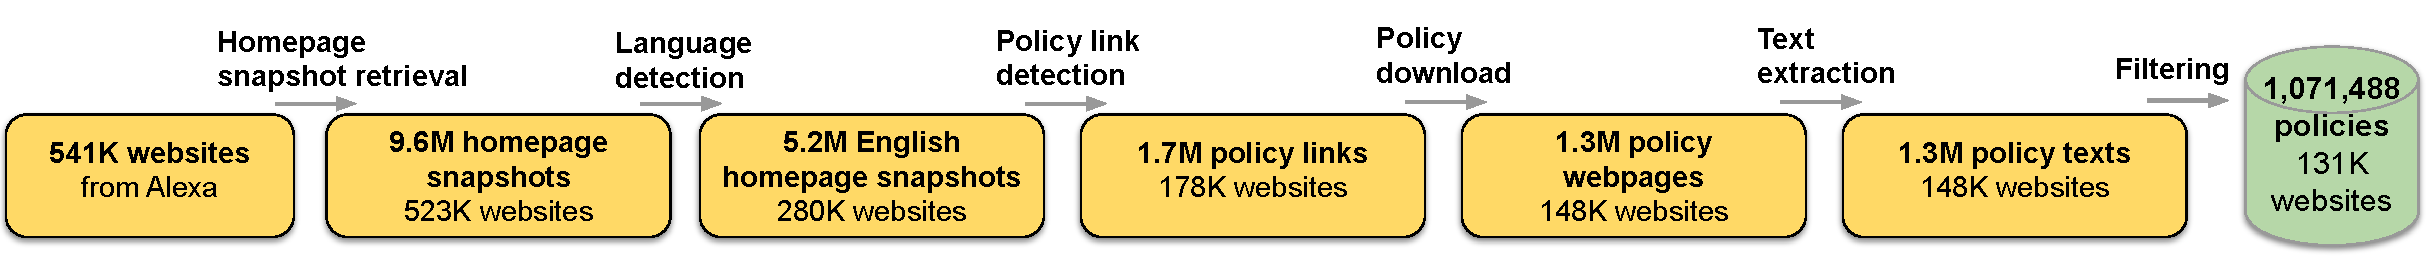
\includegraphics[width=0.99\textwidth]{chapters/privacypolicies/figures/data-collection-pipeline.pdf}
\caption[Overview of the data collection steps]{Overview of the data collection steps.}
%\Description[Data Collection Pipeline]{A flow diagram for our data collection pipeline. First we collect 541K websites from Alexa. Then we collect 9.6M homepage snapshots from 523K of those websites. We reduce this to 5.2M English homepage snapshots from 280K websites. We find 1.7M documents with privacy policy links from 178K websites. We find 1.3M privacy policy webpages from 148K websites. We extract text from 1.3M of those. Then we filter, leaving us with 1,071,488 policies from 131K websites.}
\label{fig:data-collection}
\end{figure*}

\subsection{Building the list of target websites}
\label{subsec:ppot:building-website-list}
We began by identifying a set of websites to include in our data collection process.
We chose websites that appeared in the Alexa top 100K list between 2009 and 2019. We considered 100K websites to be sufficient to reach into the long tail of the web, yet not so numerous as to pose computational challenges for data collection or analysis.

Next, we selected a method for discretizing time windows in our longitudinal dataset. We struck a trade-off between enabling granular analysis and limiting computational and storage requirements. For each website, we retrieved one snapshot from the first half of the year (January-June), and one from the second half (July-December). We call these six-month time spans~\emph{intervals}, and we use intervals as the basic time unit of our data collection and analysis. We refer to the first interval in a year as ``A'' and the second as ``B,'' so the first half of 2005 is ``2005A.''
For each interval, we used the daily archives of the Alexa top million list~\cite{naab2019prefix} to retrieve the Alexa rankings closest to the interval's midpoint: either March 31 (A) or September 30 (B).
We collected the Alexa ranks for each interval from the beginning of Alexa’s publication in 2009 to 2019.
We obtained 541,616 websites by combining all domains that appear in the top 100K of these 22 Alexa lists (two lists per year for 11 years).

\subsection{Building the list of snapshots}
\label{subsec:ppot:snapshot-retrieval}
Next, we determined the list of homepage snapshots available on the Wayback Machine
by querying their \emph{CDX Server API}~\cite{wayback-cdx-api}.
When a website had multiple snapshots in a six-month interval, we picked the snapshot closest to the midpoint of the interval.
We did not restrict our queries to a time window when searching for snapshots.
For instance, if {\tt example.com} was only listed in the Alexa top 100K in 2019,
we included its snapshots from any other year including as early as 1996, the first year for which Internet Archive has crawls~\cite{WaybackMachineGeneralInformation}.

\subsection{Downloading privacy policies}
\label{subsec:ppot:download-policies}
To download archived privacy policies, we built a custom crawler based on 
\emph{Pyppeteer}~\cite{miyakogi2019May}.


{\textbf{Language detection.}}
We limited ourselves to privacy policies in English, because our work is motivated by U.S. and EU developments and because evaluating privacy policies in other languages would require additional language proficiency. To exclude non-English websites from our crawls, we ran a language detection crawl that loaded the most recent homepage snapshot of each website, extracted the page text and identified the language of the extracted text using the \emph{Polyglot} Python library~\cite{polyglot-pypi}. If the latest snapshot failed to load, we tried to visit up to three random homepage snapshots to identify the site's language. 
We identified 280,798 English websites (5,223,228 snapshots),
and discarded the remaining 243,060 websites.


{\textbf{Loading the homepage snapshot.}}
To download archived privacy policies, we first loaded the homepage snapshot and ran a second language check to make sure the snapshot was in English to account for changes in ownership or localization.
Second, we aborted visits where the crawler attempted to load the live (non-archived) version of the page or a snapshot from another interval due to a redirection.
Finally, we monitored all requests that the crawler made and blocked requests that attempted to fetch resources from live websites.

{\textbf{Privacy policy link detection.}}
Privacy policy links are not universally standardized in their text or URL.
We chose to use \textit{link texts}---that is, the clickable text appearing within the \texttt{<a>} element---to detect privacy policy links over other link features such as the URL path. Link texts are expected to be recognizable by users, and therefore more likely to contain certain keywords.

We detected policy links using exact and partial keyword matching.
We compiled these terms based on prior research~\cite{libert2018automated} and adding other terms by manually analyzing a sample of 100 pages where we did not find a privacy policy link in a pilot crawl. 
The manual analysis of these pages involved searching for privacy policy links and checking whether the linked page’s title, headers and content described a privacy policy or not. 

The link detection method is designed to be comprehensive and may lead to pages that do not contain actual privacy policies.
We detected and removed these false positives after the crawl (Section~\ref{sec:ppot:classifier}).

{\textbf{Policy download.}}
For each detected privacy policy link, we queried the Wayback Machine CDX API to retrieve the list of snapshots that were in the same time interval as the homepage snapshot. 
If the link URL ended in ``.pdf,'' we used the Python \textit{requests} library~\cite{PyPI-requests} to retrieve the document.
If the link URL did not end in ``.pdf,'' we loaded the policy snapshot URL using the Pyppeteer-based crawler and ran a final language check to eliminate non-English policies.

{\textbf{Boilerplate removal and text extraction.}}
Privacy policy webpages typically include \emph{boilerplate} content that is separate from the policy (e.g., sidebars, footers, and headers). 
We removed boilerplate and extracted the main article from the page's DOM using the standalone version of Mozilla’s \emph{Readability} library~\cite{readability-mozilla}. 
Next, we extracted Markdown formatted text from the \emph{readable} policy web page using the \emph{html2text} Python library~\cite{html2text-github}. Markdown formatting allowed us to retain the links and basic document structure such as headers and lists, with minimal markup overhead.

\subsection{Practical and ethical considerations}
\label{subsec:ppot:practical-matters}
We confirmed that the Internet Archive’s terms of use do not prohibit automated access. Prior to starting our crawls, we sent an email to the IA’s contact address to notify them of our study.
We note that several prior works used Wayback Machine~\cite{lerner2016internet, lerner2017rewriting,brunelle2015not,brunelle2016impact}.

We took steps to minimize any adverse impact of our crawl on the Wayback Machine’s servers.
To reduce our bandwidth footprint, we disabled image downloads and limited the number of parallel crawl workers to 256.
We slowed down our crawls by pausing the workers when they received HTTP 429 (``Too Many Requests'') or HTTP 503 (``Service Unavailable'') errors from the Wayback Machine. 
After starting the crawl, we monitored the Wayback Machine server load stats~\cite{Wayback-Stats} to ensure that we were not imposing a significant load.

\subsection{Evaluating data quality}
\label{subsec:ppot:failure-analysis}

To ensure our dataset was of high quality, we manually investigated causes of failure (i.e., homepages where the crawler did not extract privacy policy text). We started with 5,223,228 homepage snapshots, and our crawler was able to download 1,292,420 privacy policy snapshots (24\%).
Downloads of privacy policies corresponding to the other 3,930,808 homepage snapshots failed due to various causes which we list in Table~\ref{tab:failure-cause}. While the high frequency of absent policies may be counter-intuitive, we found that only about 2\% of missing policies were attributable to crawler limitations.

The most common cause for a missing privacy policy, by far, was the crawler loading an archived homepage but failing to identify a privacy policy link.
The next most common cause was a~\emph{blank homepage}, where the crawler could not extract any text. Another recurring issue was that, though we had attempted to filter our non-English sites before the crawl, some homepage snapshots were classified as non-English.

To investigate the root causes of crawler failures, we manually analyzed 100 random snapshots for each of the most common crawl failures.
The main takeaways are:
only 4 of 100 homepages where the crawler did not identify a privacy policy link actually had a privacy policy link. Only 3 of 100 homepages detected as \emph{blank} contained a privacy policy link, while 13 contained some text in a separate frame--- typically old webpages. We further explore the relation between the snapshot age and crawl success in 
Section~\ref{subsec:ppot:data-overview}.

In sum, the overwhelming majority of crawl failures were attributable to homepage snapshots that did not contain a policy link, were not archived by the Wayback Machine (e.g., due to \texttt{robots.txt} rules), or were in a language other than English. The missing privacy policies that are attributable to limitations of the crawler are about 2\% of all snapshots (4\% of 44.7\% + 3\% of 7.3\%).


\begin{table}[t]
\centering
\resizebox{0.9\columnwidth}{!}{%
\begin{tabular}{@{}lrr@{}}
\toprule
\textbf{Failure cause}                           & \textbf{Count} & \textbf{Percent} \\ \midrule
No privacy policy link found on homepage         & 2,336,849      & 44.7\%       \\
Homepage detected as blank                        & 383,337       & 7.3\%      \\
Non-English homepage                             & 310,563        & 5.9\% \\
Policy page is not archived in this interval     & 271,736        & 5.2\%\\
Out-of-interval redirection for homepage         & 158,727        & 3.0\%\\
\bottomrule
\end{tabular}%
}
\caption{The five most common causes for the crawler to not download a privacy policy for a homepage. Out-of-interval redirection (row 5) means our crawler was redirected by the Wayback Machine to a snapshot in a different interval.}
\label{tab:failure-cause}
\end{table}

